% !Mode:: "TeX:UTF-8"
% !TEX program = xelatex
\section{Question 1}
\begin{equation*}
    \begin{aligned}
        \EE\中括号{\log\小括号{\frac{S(n\delta t)}{S_0}}} &= \EE\中括号{n\log d+\log\小括号{\frac{u}{d}}\sum_{i=1}^nR_i} \\
        &= n\log d + \log\小括号{\frac{u}{d}}\sum_{i=1}^n\EE\中括号{R_i} \\
        &= n\log d + \log\小括号{\frac{u}{d}}\sum_{i=1}^np \\
        &= n\log d + \log\小括号{\frac{u}{d}}np
    \end{aligned}
\end{equation*}

\begin{equation*}
    \begin{aligned}
        \var\中括号{\log\小括号{\frac{S(n\delta t)}{S_0}}} &= \var\中括号{n\log d+\log\小括号{\frac{u}{d}}\sum_{i=1}^nR_i} \\
        &= \var\中括号{\log\小括号{\frac{u}{d}}\sum_{i=1}^nR_i} \\
        &= \小括号{\log\小括号{\frac{u}{d}}}^2\sum_{i=1}^n\var\小括号{R_i} \\
        &= \小括号{\log\小括号{\frac{u}{d}}}^2\sum_{i=1}^nnp(1-p)
    \end{aligned}
\end{equation*}



\section{Question 2}
\subsection{Review}
The three papers discussed the method of estimating option prices by simulations. Boyle's paper first introduced the how to use Monte Carlo method to solve option valuation problems, he suggested that we can first generate the returns of the stock and then calculate the option value based on the risk neutrality assumption. 19 years later, Broadie and Glasserman presented two direct method for estimating option prices by simulation, including pathwise method and likelihood ration method. The two methods raise the computational speed and return unbiased estimates. In 2001, F.A.Longstaff and E.S.Schwartz extended the method to American options. The key is to use least squares to estimate the conditional expected payoff, which satisfy the situation where FDM can not be used, such as valuation of American options.


\subsection{From Binomial to Trinomial Method}
It's possible if the process allow the stock price at a time point equal to the price at previous time point for a given probability.

Then the trinomial tree is like the form according to Figure~\ref{F:trinomial-tree}, and it has parameters $u$, $d$, $p_1$, $p_2$, $M$.
\begin{figure}
    \centering
    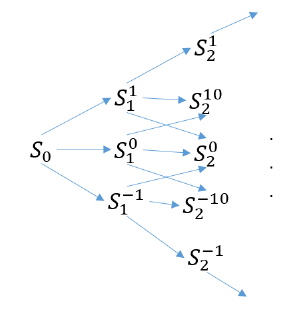
\includegraphics[width=.5\textwidth]{figures/2019-12-25-trinomial-tree.png}
    \caption{Trinomial Tree}\label{F:trinomial-tree}
\end{figure}


\subsection{Appendix}
\paragraph{Paper I:} Phelim P. Boyle, \emph{Options: A Monte Carlo approach}\footnote{Journal of Financial Economics, Volume 4, Issue 3, 1977.}.

Abstract: This paper develops a Monte Carlo simulation method for solving option valuation problems. The method simulates the process generating the returns on the underlying asset and invokes the risk neutrality assumption to derive the value of the option. Techniques for improving the efficiency of the method are introduced. Some numerical examples are given to illustrate the procedure and additional applications are suggested.

\paragraph{Paper II:} Mark Broadie, Paul Glasserman, \emph{Estimating Security Price Derivatives Using Simulation}\footnote{Management Science, Volume 42, No. 2 1996.}.

Abstract: Simulation has proved to be a valuable tool for estimating security prices for which simple closed form solutions do not exist. In this paper we present two direct methods, a pathwise method and a likelihood ratio method, for estimating derivatives of security prices using simulation. With the direct methods, the information from a single simulation can be used to estimate multiple derivatives along with a security's price. The main advantage of the direct methods over resimulation is increased computational speed. Another advantage is that the direct methods give unbiased estimates of derivatives, whereas the estimates obtained by resimulation are biased. Computational results are given for both direct methods, and comparisons are made to the standard method of resimulation to estimate derivatives. The methods are illustrated for a path independent model (European options), a path dependent model (Asian options), and a model with multiple state variables (options with stochastic volatility).

\paragraph{Paper III:} Francis A. Longstaff, Eduardo S. Schwartz, \emph{Valuing American Options by Simulation: A Simple Least­Squares Approach}\footnote{The Review of Financial Studies, Volume 14, Issue 1, 2001.}.

Abstract: This article presents a simple yet powerful new approach for approximating the value of American options by simulation. The key to this approach is the use of least squares to estimate the conditional expected payoff to the optionholder from continuation. This makes this approach readily applicable in path­dependent and multifactor situations where traditional finite difference techniques cannot be used. We illustrate this technique with several realistic examples including valuing an option when the underlying asset follows a jump­diffusion process and valuing an American swaption in a 20­factor string model of the term structure.
